% ========================================================================
% INSTITUTO FEDERAL DO PIAUÍ - IFPI CAMPUS FLORIANO
% TEMPLATE DE PROJETO DE PESQUISA (ABNT NBR 15287 / MANUAL IFPI 2024)
% ========================================================================
% Este arquivo é a matriz principal do seu Projeto de Pesquisa.
% A estrutura é modular e importa os arquivos das pastas config/ e estrutura/.
%
% Conforme a ABNT NBR 14724:2024 (item 4.2.2), NBR 6024 e o Manual do IFPI,
% o trabalho é organizado exclusivamente em SEÇÕES (primárias, secundárias,
% terciárias, quaternárias e quinárias) e não em capítulos.
% ========================================================================

% ========================================================================
% CONFIGURAÇÕES E METADADOS
% ========================================================================
\documentclass[
    12pt,        % Tamanho da fonte principal
    openany,     % Seções iniciam em qualquer página
    oneside,     % Impressão apenas frente
    a4paper,     % Formato A4
    english,     % Idioma adicional
    french,      % Idioma adicional
    spanish,     % Idioma adicional
    brazil,      % Idioma principal
    article      % Estruturação por seções (sem \chapter) conforme NBR 14724:2024
]{abntex2}

\input{config/config}   % configurações de formatação
% ========================================================================
% DADOS DO PROJETO DE PESQUISA
% Edite os valores abaixo para personalizar o template.
% ========================================================================

% Instituição e identificação do curso
\instituicao{Instituto Federal de Educação, Ciência e Tecnologia do Piauí}
\campus{Campus Floriano}
\curso{Tecnologia em Análise e Desenvolvimento de Sistemas}
\areaconcentracao{} % Opcional: defina a área de concentração ou deixe vazio

% Título e autoria
\titulo{TÍTULO DO PROJETO DE PESQUISA}
\subtitulo{SUBTÍTULO SE HOUVER}
\tituloestrangeiro{} % Título traduzido (ex: em inglês para o abstract)
\autor{NOME COMPLETO DO AUTOR}
\emailautor{autor@aluno.ifpi.edu.br}
\vinculoautor{IFPI -- Campus Floriano}

% Orientação
\orientador{Prof. Me. Ronaldo Pires Borges}
\emailorientador{ronaldo.borges@ifpi.edu.br}
\vinculoorientador{IFPI -- Campus Floriano} % Vínculo do orientador

% Coorientação (deixe vazio se não houver coorientador)
\coorientador{}
\emailcoorientador{}
\vinculocoorientador{}

% Informações gerais
\local{Floriano -- PI}
\data{2026}
\dataaprovacao{XX/XX/XXXX} % ESCREVA A DATA DA BANCA / APROVAÇÃO

% Descrição apresentada na folha de rosto
\preambulo{Projeto de pesquisa apresentado ao Instituto Federal de Educação, Ciência e Tecnologia do Piauí -- Campus Floriano, como requisito para aprovação na disciplina de Projeto de Pesquisa do curso de Tecnologia em Análise e Desenvolvimento de Sistemas.}

% Natureza do trabalho
% \naturezatrabalho{Projeto de pesquisa apresentado ao Instituto Federal de Educação, Ciência e Tecnologia do Piauí como requisito para aprovação...}

% Grau pretendido (opcional)
% \grau{Tecnólogo em Análise e Desenvolvimento de Sistemas} 

% ========================================================================
% INSTRUÇÕES RÁPIDAS
% - Substitua os textos pelos dados reais da sua pesquisa.
% - Campos opcionais sem uso podem permanecer vazios.
% ========================================================================
 % dados institucionais e do projeto

% ========================================================================
% INÍCIO DO DOCUMENTO
% ========================================================================

\begin{document}
% Seleciona o idioma do documento (conforme pacotes do babel)
\selectlanguage{brazil}
% Retira espaço extra obsoleto entre as frases
\frenchspacing

% ========================================================================
% ELEMENTOS PRÉ-TEXTUAIS
% ========================================================================
\input{estrutura/pre_textuais}

% ========================================================================
% ELEMENTOS TEXTUAIS
% ========================================================================

\section{INTRODUÇÃO}
\label{sec:introducao}

A introdução de um projeto de pesquisa deve apresentar o tema de forma clara e contextualizada, demonstrando sua relevância no cenário atual. Conforme o \citeonline{IFPI_Manual_2024}, esta seção tem como objetivo situar o leitor no contexto da investigação, apresentando a problematização, a justificativa e a delimitação do objeto de estudo.

Em conformidade estrita com a ABNT NBR 14724:2024 (item 4.2.2) e o Manual de Normalização do IFPI (2024), os trabalhos acadêmicos são estruturados exclusivamente em \textbf{seções} e não em capítulos. 

O tema desta pesquisa insere-se no campo de [ÁREA DE CONHECIMENTO], especificamente abordando [TEMA ESPECÍFICO]. A escolha deste tema justifica-se pela [JUSTIFICATIVA INICIAL], considerando sua relevância tanto no âmbito acadêmico quanto na aplicação prática.

Segundo \citeonline{marconi2017}, a área de [ÁREA DE CONHECIMENTO] tem apresentado crescente interesse por estudos que abordem [ASPECTO RELEVANTE DO TEMA]. Esta tendência evidencia a necessidade de pesquisas que contribuam para o avanço do conhecimento nesta área, com embasamento teórico fundamentado por autores clássicos como \citeonline{creswell2018} e \citeonline{gil2019}.

Uma alteração fundamental trazida pela norma ABNT NBR 10520:2023 determina o uso de caixa mista (primeira letra maiúscula e demais minúsculas) nas chamadas de autor inseridas entre parênteses, por exemplo \cite{marconi2017}, diferentemente da norma antiga que exigia caixa alta.


\subsection{PROBLEMA DE PESQUISA}
\label{subsec:problema}

O problema de pesquisa constitui o elemento central que orienta todo o desenvolvimento do estudo. Conforme \citeonline{gil2019}, um problema bem formulado deve ser claro, preciso e operacional, permitindo a definição de objetivos específicos e a escolha de métodos adequados para sua investigação.

No contexto desta pesquisa, observa-se que [DESCRIÇÃO DO PROBLEMA IDENTIFICADO]. Esta situação tem gerado [CONSEQUÊNCIAS OU IMPACTOS DO PROBLEMA], evidenciando a necessidade de estudos que possam contribuir para sua compreensão e possível solução.

Diante do exposto, formula-se o seguinte problema de pesquisa:

\textbf{[PERGUNTA DE PESQUISA PRINCIPAL]?}

Este questionamento surge da observação de que [CONTEXTUALIZAÇÃO DO PROBLEMA], conforme evidenciado por \citeonline{silva2023} em seus estudos sobre [ÁREA RELACIONADA].


\subsection{HIPÓTESES}
\label{subsec:hipoteses}   

As hipóteses representam respostas provisórias ao problema de pesquisa, baseadas no conhecimento teórico disponível e na experiência do pesquisador. Segundo \citeonline{marconi2017}, as hipóteses devem ser testáveis e formuladas de maneira clara e precisa.

Para o problema apresentado, formulam-se as seguintes hipóteses:

\textbf{Hipótese Principal (H1):} [HIPÓTESE PRINCIPAL DA PESQUISA]

\textbf{Hipóteses Secundárias:}
\begin{itemize}
    \item \textbf{H2:} [SEGUNDA HIPÓTESE]
    \item \textbf{H3:} [TERCEIRA HIPÓTESE, SE APLICÁVEL]
\end{itemize}

Essas hipóteses serão testadas através da metodologia proposta, permitindo confirmar ou refutar as suposições iniciais da pesquisa.


\subsection{OBJETIVOS}
\label{subsec:objetivos}

Os objetivos definem o que se pretende alcançar com a realização da pesquisa. Devem ser formulados de forma clara e precisa, utilizando verbos no infinitivo que expressem ações concretas e mensuráveis.

\subsubsection{Objetivo Geral}
\label{subsubsec:objetivo-geral}

[DESCREVER O OBJETIVO GERAL DA PESQUISA, UTILIZANDO VERBO NO INFINITIVO E EXPRESSANDO DE FORMA CLARA O QUE SE PRETENDE ALCANÇAR COM O ESTUDO]

\subsubsection{Objetivos Específicos}
\label{subsubsec:objetivos-especificos}

\begin{enumerate}
    \item Objetivo específico 1;
    \item Objetivo específico 2;
    \item Objetivo específico 3;
    \item Objetivo específico 4 (se aplicável).
\end{enumerate}


\subsection{JUSTIFICATIVA}
\label{subsec:justificativa}

A justificativa deve demonstrar a relevância e a importância da pesquisa, apresentando argumentos que evidenciem sua contribuição para o avanço do conhecimento científico e/ou para a solução de problemas práticos.

Esta pesquisa justifica-se por diversos aspectos:

\textbf{Relevância Científica:} O tema abordado contribui para o avanço do conhecimento na área de [ÁREA DE CONHECIMENTO], especialmente no que se refere a [ASPECTO ESPECÍFICO]. Conforme destacado por \citeonline{inep2022}, existe uma lacuna na literatura sobre [LACUNA IDENTIFICADA], que esta pesquisa pretende contribuir para preencher.

\textbf{Relevância Social:} Os resultados desta pesquisa poderão beneficiar [PÚBLICO-ALVO OU SOCIEDADE EM GERAL], uma vez que [EXPLICAR COMO OS RESULTADOS PODEM SER APLICADOS]. Segundo dados de \cite{instituicao2023}, [APRESENTAR DADOS QUE EVIDENCIEM A RELEVÂNCIA SOCIAL].

\textbf{Relevância Acadêmica:} Este estudo contribuirá para a formação acadêmica do pesquisador e para o desenvolvimento de pesquisas futuras na área, fornecendo subsídios teóricos e metodológicos para estudos similares.

\textbf{Viabilidade:} A pesquisa é viável considerando os recursos disponíveis, o tempo previsto para sua execução e o acesso às fontes de informação necessárias.


\section{REFERENCIAL TEÓRICO}
\label{sec:referencial}

O referencial teórico constitui a base conceitual da pesquisa, apresentando as teorias, conceitos e estudos que fundamentam a investigação. Conforme exposto por \citeonline{IFPI_Manual_2024}, esta seção destina-se a detalhar as leituras e embasamentos teóricos que sustentam a proposta, explicando, classificando e demonstrando o estado da arte do objeto de estudo.

\subsection{CONCEITOS FUNDAMENTAIS}
\label{subsec:fundamentacao1}

Aqui você deve escrever e citar autores que embasarão teoricamente o projeto. Para citações no texto, utilize \verb|\citeonline{chave}| para o formato autor no texto, como \citeonline{creswell2018}, ou \verb|\cite{chave}| para citações entre parênteses \cite{gil2019}.

\subsubsection{Normalização Científica e Tipografia}
\label{subsubsec:normalizacao}

Conforme a ABNT NBR 6024 e o Manual do IFPI (2024), a numeração progressiva e a formatação tipográfica dos títulos das seções devem obedecer rigorosamente a uma hierarquia estabelecida.

\paragraph{Citações e Regras da ABNT}
\label{para:citacoes}

As seções quaternárias (criadas com o comando \verb|\paragraph{}|) são formatadas com fonte em caixa baixa (inicial maiúscula) e estilo itálico.

\subparagraph{Diretrizes Específicas do IFPI}
\label{subpara:diretrizes}

As seções quinárias (criadas com o comando \verb|\subparagraph{}|) utilizam fonte em caixa baixa (inicial maiúscula) com estilo regular (sem negrito e sem itálico).

\begin{figure}[htbp]
    \centering
    \caption{Exemplo de figura no documento}
    
\includegraphics[width=0.3\textwidth]{img/Logo-IFPI-Floriano-Horizontal.png}
    \fonte{IFPI -- Instituto Federal do Piauí.}
    \label{fig:exemplo}
\end{figure}

Quando elementos visuais forem inseridos no texto, devem ser obrigatoriamente identificados e mencionados no corpo do trabalho, utilizando o comando \verb|\autoref{}|. Conforme orienta a \citeonline{ABNT_NBR14724_2011}, esses elementos devem ser citados por seu número e título. Assim, faz-se referência à \autoref{fig:exemplo}, na qual se apresenta a logomarca do IFPI Campus Floriano.


% ========================================================================
% CITAÇÃO DIRETA LONGA - EXEMPLO
% ========================================================================
\begin{citacao}
Quando uma citação direta ultrapassa três linhas do texto original, ela deve ser apresentada em destaque, com recuo especial de 4 cm da margem esquerda, sem o uso de aspas, utilizando fonte menor e espaçamento simples entre as linhas. Esta formatação diferenciada permite ao leitor identificar claramente a reprodução literal da fonte \cite{ABNT_NBR10520_2023}.
\end{citacao}

\subsection{ESTUDOS RELACIONADOS}
\label{subsec:estudos-relacionados} 

Esta seção apresenta uma revisão dos principais estudos relacionados ao tema da pesquisa, evidenciando o estado da arte e identificando lacunas.

A \textbf{tabela} é uma forma não discursiva de apresentação em que o dado numérico é central (normas do IBGE). Deve apresentar estrutura aberta (sem bordas verticais laterais ou fechamento inferior) e cabeçalho demarcado por linhas horizontais \cite{ABNT_NBR14724_2011,ABNT_NBR15287_2011}. A \autoref{tab:estudos} exemplifica a formatação adequada de uma tabela usando o pacote \texttt{booktabs}.

\begin{table}[htbp]
    \centering
    \caption{Exemplo de tabela com dados numéricos (Padrão IBGE)}
    \label{tab:estudos}
    \begin{tabularx}{0.8\textwidth}{p{4cm}XX}
        \toprule
        \textbf{Estudo} & \textbf{Amostra} & \textbf{Métrica principal} \\
        \midrule
        Costa e Rocha (2023) & 120 respondentes & Média de adoção = 4,1 \\
        Silva e Santos (2023) & 18 escolas analisadas & Taxa de conclusão = 87\% \\
        Souza (2021) & 32 entrevistas & Índice de concordância = 0,74 \\
        \bottomrule
    \end{tabularx}
    \fonte{Elaborado pelo autor a partir dos estudos revisados.}
\end{table}

O \textbf{quadro}, diferentemente da tabela, apresenta dados qualitativos. Possui estrutura fechada em todos os lados (normas ABNT). O \autoref{qua:estudos} exemplifica a formatação adequada de um quadro.

\begin{quadro}[htbp]
    \centering
    \caption{Exemplo de quadro com conteúdo qualitativo (Padrão ABNT)}
    \label{qua:estudos}
    \begin{tabularx}{\textwidth}{|p{3cm}|p{4cm}|X|}
        \hline
        \textbf{Autor/Ano} & \textbf{Metodologia} & \textbf{Principais Resultados} \\
        \hline
        Autor A (2023) & Pesquisa quantitativa & Ênfase na mensuração de impacto tecnológico \\ \hline
        Autor B (2022) & Estudo de caso & Identifica barreiras institucionais para inovação \\ \hline
        Autor C (2021) & Pesquisa qualitativa & Discute competências desenvolvidas pelos participantes \\ \hline
    \end{tabularx}
    \fonte{Elaborado pelo autor.}
\end{quadro}

A aplicação do efeito zebrado (\textit{zebra striping}) melhora a legibilidade visual das informações. No LaTeX, essa formatação é obtida ativando o pacote \texttt{xcolor} (opção \texttt{[table]}) e aplicando o comando \verb|\rowcolors{2}{gray!15}{white}|. A \autoref{tab:estudos_zebrada} e o \autoref{qua:estudos_zebrado} demonstram esse recurso visual.

\begin{table}[htbp]
    \centering
    \caption{Exemplo de tabela numérica com efeito zebrado}
    \label{tab:estudos_zebrada}
    \rowcolors{2}{gray!15}{white}
    \begin{tabularx}{0.8\textwidth}{p{4cm}XX}
        \toprule
        \textbf{Estudo} & \textbf{Amostra} & \textbf{Métrica principal} \\
        \midrule
        Costa e Rocha (2023) & 120 respondentes & Média de adoção = 4,1 \\
        Silva e Santos (2023) & 18 escolas analisadas & Taxa de conclusão = 87\% \\
        Souza (2021) & 32 entrevistas & Índice de concordância = 0,74 \\
        \bottomrule
    \end{tabularx}
    \fonte{Elaborado pelo autor a partir dos estudos revisados.}
\end{table}

\begin{quadro}[htbp]
    \centering
    \caption{Exemplo de quadro qualitativo com efeito zebrado}
    \label{qua:estudos_zebrado}
    \rowcolors{2}{gray!15}{white}
    \begin{tabularx}{\textwidth}{|p{3cm}|p{4cm}|X|}
        \hline
        \textbf{Autor/Ano} & \textbf{Metodologia} & \textbf{Principais Resultados} \\
        \hline
        Autor A (2023) & Pesquisa quantitativa & Ênfase na mensuração de impacto tecnológico \\ \hline
        Autor B (2022) & Estudo de caso & Identifica barreiras institucionais para inovação \\ \hline
        Autor C (2021) & Pesquisa qualitativa & Discute competências desenvolvidas pelos participantes \\ \hline
    \end{tabularx}
    \fonte{Elaborado pelo autor.}
\end{quadro}

Recomenda-se o uso da ferramenta online \textit{Tables Generator}\footnote{https://www.tablesgenerator.com/} para estruturar tabelas e quadros visualmente antes da inclusão no código LaTeX.


\section{METODOLOGIA}
\label{sec:metodologia}

A metodologia descreve detalhadamente os procedimentos que serão adotados para a realização da pesquisa. O texto deve manter um tratamento impessoal e objetivo em conformidade com o \citeonline{IFPI_Manual_2024}.

\subsection{CARACTERIZAÇÃO DA PESQUISA}
\label{subsec:caracterizacao}

Esta pesquisa pode ser caracterizada, quanto aos seus objetivos, como EXPLORATÓRIA, uma vez que busca proporcionar maior familiaridade com o problema. Segundo \citeonline{gil2019}, pesquisas dessa natureza têm como objetivo o aprimoramento de ideias ou a descoberta de intuições.

Quanto à abordagem, trata-se de uma pesquisa QUANTITATIVA, pois adota métodos estatísticos para mensurar os dados coletados. \citeonline{creswell2018} destaca que a abordagem mista ou quantitativa é adequada quando se pretende testar teorias objetivas examinando a relação entre variáveis.

Em relação aos procedimentos técnicos, será realizada uma PESQUISA BIBLIOGRÁFICA, que, conforme \citeonline{marconi2017}, caracteriza-se pelo levantamento de contribuições teóricas já publicadas sobre o tema.

\begin{figure}[htbp]
    \centering
    \caption{Esquema metodológico da pesquisa}
    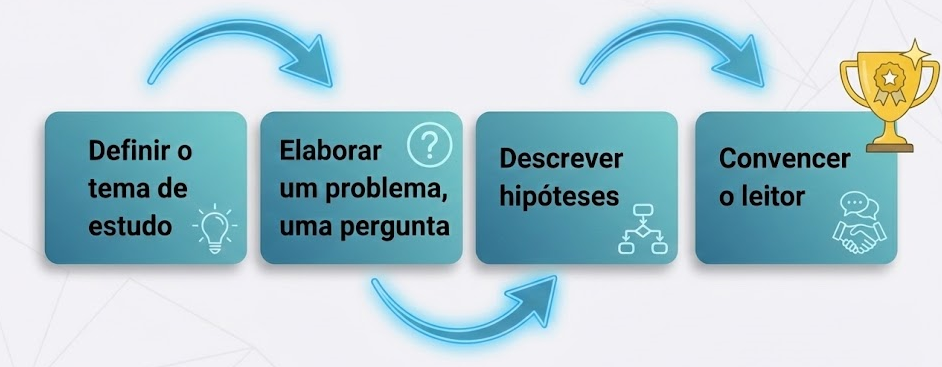
\includegraphics[width=0.85\textwidth]{img/tema do tcc.png}
    \fonte{Adaptado de \citeonline{Moretti_ComoEscolherTemaTCC_2024}}
    \label{fig:esquema_metodologico}
\end{figure}

\subsection{POPULAÇÃO E AMOSTRA}
\label{subsec:populacao-amostra}

A população desta pesquisa é constituída por [DEFINIR A POPULAÇÃO]. Para a definição da amostra, será utilizada a técnica de [TIPO DE AMOSTRAGEM], que, segundo \citeonline{hair2019}, é adequada para garantir a representatividade dos dados.

O tamanho da amostra foi calculated considerando [CRITÉRIOS DE CÁLCULO], resultando em [NÚMERO] participantes/elementos.

\subsection{TÉCNICAS DE COLETA DE DADOS}
\label{subsec:coleta-dados}

A coleta de dados será realizada através de [INSTRUMENTOS DE COLETA], que permitirão obter informações sobre [TIPO DE INFORMAÇÕES].

Os instrumentos escolhidos foram:
\begin{itemize}
    \item \textbf{[INSTRUMENTO 1]:} [DESCRIÇÃO E JUSTIFICATIVA];
    \item \textbf{[INSTRUMENTO 2]:} [DESCRIÇÃO E JUSTIFICATIVA].
\end{itemize}

\subsection{ANÁLISE DOS DADOS}
\label{subsec:analise-dados}

Os dados coletados serão analisados utilizando [TÉCNICAS DE ANÁLISE]. Para dados quantitativos, utilizar-se-á estatística descritiva e inferencial. Os dados qualitativos serão submetidos à análise de conteúdo.

\subsection{ASPECTOS ÉTICOS}
\label{subsec:aspectos-eticos}

Esta pesquisa será desenvolvida respeitando os princípios éticos estabelecidos pela Resolução nº 466/2012 do Conselho Nacional de Saúde. [SE APLICÁVEL: O projeto será submetido ao Comitê de Ética em Pesquisa (CEP) antes da coleta de dados]. Todos os participantes assinarão o Termo de Consentimento Livre e Esclarecido (TCLE).


\section{RESULTADOS ESPERADOS}
\label{sec:resultados-esperados}

Os resultados esperados descrevem os produtos, impactos e transformações que a pesquisa pretende alcançar, devendo alinhar-se aos objetivos propostos:

\begin{itemize}
    \item \textbf{Impactos científicos}: [CONTRIBUIÇÃO PARA O AVANÇO TEÓRICO DA ÁREA];
    \item \textbf{Impactos tecnológicos/sociais}: [MUDANÇAS ESPERADAS NO CONTEXTO PRÁTICO];
    \item \textbf{Produtos e entregáveis}: [LISTAR RELATÓRIOS, SOFTWARES OU ARTIGOS GERADOS];
    \item \textbf{Indicadores de acompanhamento}: [DEFINIR MÉTRICAS E METAS DE AVALIAÇÃO].
\end{itemize}


\section{RECURSOS}
\label{sec:recursos}

Esta seção discrimina os recursos necessários para viabilizar a execução do projeto, conforme orientação da NBR 15287.

\subsection{RECURSOS HUMANOS}
\label{subsec:recursos-humanos}

[DESCREVER A EQUIPE ENVOLVIDA: PESQUISADOR PRINCIPAL, ORIENTADOR, COORIENTADOR E COLABORADORES, DESTACANDO AS ATIVIDADES DE CADA UM].

\subsection{RECURSOS MATERIAIS E INFRAESTRUTURAIS}
\label{subsec:recursos-materiais}

[DETALHAR INFRAESTRUTURA DE LABORATÓRIOS, EQUIPAMENTOS, SOFTWARES E INSUMOS NECESSÁRIOS].

\subsubsection{Orçamento}
\label{subsubsec:orcamento}

A \autoref{tab:orcamento} sintetiza os custos previstos por categoria de despesa para a realização da pesquisa.

\begin{table}[htbp]
    \centering
    \caption{Orçamento estimado da pesquisa}
    \label{tab:orcamento}
    \begin{tabularx}{0.85\textwidth}{Xcr}
        \toprule
        \textbf{Item / Descrição} & \textbf{Qtd.} & \textbf{Valor Total (R\$)} \\
        \midrule
        Material de escritório e insumos & 1 & 150,00 \\
        Impressões e cópias de questionários & 1 & 100,00 \\
        Deslocamento e transporte para coleta & 1 & 200,00 \\
        Licenças de software e ferramentas & 1 & 300,00 \\
        \midrule
        \textbf{TOTAL} & & \textbf{750,00} \\
        \bottomrule
    \end{tabularx}
    \fonte{Elaborado pelo autor.}
\end{table}


\section{CRONOGRAMA DE EXECUÇÃO}
\label{sec:cronograma}

O cronograma apresenta a distribuição temporal das atividades previstas para a realização da pesquisa. O \autoref{qua:cronograma} detalha as etapas e seus respectivos meses de execução.

\begin{quadro}[htbp]
    \centering
    \caption{Cronograma de execução da pesquisa}
    \label{qua:cronograma}
    \begin{tabularx}{\textwidth}{|X|c|c|c|c|c|c|}
        \hline
        \textbf{Atividades} & \textbf{Jan} & \textbf{Fev} & \textbf{Mar} & \textbf{Abr} & \textbf{Mai} & \textbf{Jun} \\
        \hline
        Revisão bibliográfica e estado da arte & \checkmark & \checkmark & & & & \\
        \hline
        Elaboração e validação dos instrumentos & & \checkmark & \checkmark & & & \\
        \hline
        Coleta de dados em campo & & & \checkmark & \checkmark & & \\
        \hline
        Processamento e análise dos dados & & & & \checkmark & \checkmark & \\
        \hline
        Redação do relatório final e artigo & & & & & \checkmark & \checkmark \\
        \hline
        Revisão e submissão/defesa & & & & & & \checkmark \\
        \hline
    \end{tabularx}
    \fonte{Elaborado pelo autor.}
\end{quadro}


% ========================================================================
% ELEMENTOS PÓS-TEXTUAIS
% ========================================================================
% ========================================================================
% ELEMENTOS PÓS-TEXTUAIS
% Referências, apêndices e anexos conforme ABNT NBR 14724:2024 / NBR 15287
% ========================================================================

% ========================================================================
% REFERÊNCIAS BIBLIOGRÁFICAS
% ========================================================================
\postextual

% Configura o título e imprime a bibliografia
\bibliography{referencias}

% ========================================================================
% GLOSSÁRIO (OPCIONAL)
% ========================================================================
% Descomente se necessário incluir glossário
% \glossary

% ========================================================================
% APÊNDICES (OPCIONAL)
% ========================================================================
% Descomente e personalize se houver apêndices (documentos produzidos pelo próprio autor)
% \quebrapagina
% \begin{apendicesenv}
%     % Imprime uma página indicando o início dos apêndices (opcional)
%     % \partapendices
%     
%     % ========================================================================
%     % APÊNDICE A - EXEMPLO DE APÊNDICE
%     % ========================================================================
%     \section{TÍTULO DO PRIMEIRO APÊNDICE}
%     \label{apendice:primeiro}
%     
%     Este é um exemplo de apêndice. Os apêndices são textos ou documentos elaborados pelo próprio autor, a fim de complementar sua argumentação.
%     
%     Exemplos de conteúdo para apêndices:
%     \begin{itemize}
%         \item Questionários utilizados na pesquisa
%         \item Roteiros de entrevistas
%         \item Códigos de programas desenvolvidos
%         \item Tabelas extensas com dados brutos
%     \end{itemize}
% \end{apendicesenv}

% ========================================================================
% ANEXOS (OPCIONAL)
% ========================================================================
% Descomente e personalize se houver anexos (documentos não produzidos pelo autor)
% \quebrapagina
% \begin{anexosenv}
%     % \partanexos
%     \section{TÍTULO DO PRIMEIRO ANEXO}
%     \label{anexo:primeiro}
%     Texto do anexo aqui.
% \end{anexosenv}

% ========================================================================
% FIM DO DOCUMENTO
% ========================================================================
\end{document}
